\section{Background}

\subsection{Offline Preference-Driven Multi-Objective Reinforcement Learning}
\label{sec:PDMORL}

Many real-world control problems, including energy-aware scheduling and power-performance management in HPC systems, naturally involve multiple conflicting objectives. We discussed some of these in Section~\ref{sec:Introduction}. Multi-objective reinforcement learning (MORL) formulates such problems by extending the scalar reward in standard RL to a vector-valued reward, enabling explicit reasoning over trade-offs between objectives such as performance and energy consumption.

Formally, a multi-objective Markov decision process (MOMDP) is defined as
\begin{equation}
    \mathcal{M} = \langle \mathcal{S}, \mathcal{A}, \mathcal{P}, 
    \mathbf{r}, \boldsymbol{\Omega} \rangle,
    \label{eq:MOMDP}
\end{equation}
where $\mathcal{S}$ and $\mathcal{A}$ denote the state and action spaces, $\mathcal{P}(s'\vert s,a)$ is the transition kernel, and $\mathbf{r}(s,a) \in \mathbb{R}^L$ is an $L$-dimensional reward vector. User preferences are encoded by a weight vector
\begin{equation}
    \boldsymbol{\omega} \in \boldsymbol{\Omega} = \Big\{
    \boldsymbol{\omega} \in \mathbb{R}^L_{\geq 0} \;\Big\vert\; 
    \sum^{L}_{i=1}\boldsymbol{\omega}_i = 1 \Big\},
    \label{eq:preference_weight_vector}
\end{equation}
which induces a scalarized reward via $f_{\boldsymbol{\omega}}(\mathbf{r}) = \boldsymbol{\omega}^T\mathbf{r}$.

Traditional scalarization-based MORL methods learn a separate policy for each fixed preference vector, which is inefficient when preferences change dynamically and impractical in offline settings where retraining is costly or impossible. To address this limitation, Preference-Driven Multi-Objective Reinforcement Learning (PD-MORL)~\cite{basaklar2023pdmorlpreferencedrivenmultiobjectivereinforcement} proposes learning a single universal value function that conditions on preferences and covers the entire preference space in one training phase.

\subsubsection{Multi-Objective Value Functions and Preference Conditioning}

PD-MORL extends Q-learning by defining a vector-valued Q-function $Q(s,a,\boldsymbol{\omega}) \in \mathbb{R}^L$, which estimates the expected discounted return for each objective under the preference $\boldsymbol{\omega}$. The optimal policy for any preference can then be recovered at inference time by conditioning the network on $\boldsymbol{\omega}$, eliminating the need to store multiple policies.

A scalarized distance metric over multi-objective Q-functions is 
defined as
\begin{equation}
    d(\mathbf{Q},\mathbf{Q}^{\prime}) = \sup_{s,a,\boldsymbol{\omega}} 
    \vert \boldsymbol{\omega}^{T}(\mathbf{Q}(s,a,\boldsymbol{\omega})
    -\mathbf{Q}^{\prime}(s,a,\boldsymbol{\omega}))\vert,
\end{equation}
which is a complete pseudo-metric space due to its one-to-many mapping nature. Intuitively, this metric bounds the maximum discrepancy a user may observe in the energy-runtime trade-off when switching between learned value functions, while ensuring convergence of the preference-driven Bellman operator.

\subsubsection{Preference-Driven Bellman Optimality Operator}

The PD-MORL Bellman optimality operator is defined as:
\begin{equation}
\begin{aligned}
(\mathcal{T}\mathbf{Q})(s,a,\boldsymbol{\omega})
&= \mathbf{r}(s,a)
+ \gamma \mathbb{E}_{s' \sim P(\cdot \mid s,a)} \Big[ \\
&\mathbf{Q}\!\Big(s',
\arg\max_{a' \in \mathcal{A}}
\big(S_c(\boldsymbol{\omega}, \mathbf{Q}(s',a',\boldsymbol{\omega}))
\cdot \boldsymbol{\omega}^{\top} \mathbf{Q}(s',a',\boldsymbol{\omega})
\big), \boldsymbol{\omega}\Big)\Big]
\end{aligned}
\label{eq:Bellman_equation}
\end{equation}
where $S_c(\cdot,\cdot)$ denotes the cosine similarity between the preference vector and the multi-objective Q-value:
\begin{equation}
    S_c(\boldsymbol{\omega},\mathbf{Q}) = 
    \frac{\boldsymbol{\omega}^T\mathbf{Q}}
    {\vert\vert \boldsymbol{\omega} \vert\vert \; 
    \vert\vert \mathbf{Q} \vert\vert}.
    \label{eq:cosine_function}
\end{equation}
This alignment term prevents domination by objectives with larger numerical scales, a critical issue in energy-performance optimization where metrics often differ by orders of magnitude. 
The resulting operator is shown to be a contraction under metric $d$, guaranteeing convergence to a unique fixed point corresponding to the optimal multi-objective value function.

\subsubsection{Offline Learning and the Preference Alignment Problem}

PD-MORL is well suited for offline reinforcement learning settings, where policies are learned from pre-collected system traces without further interaction with the environment. Since environment dynamics and objective-wise reward vectors are independent of user preferences, each recorded transition can be consistently reused across multiple preference vectors. PD-MORL leverages this property through hindsight experience replay, augmenting transitions $(s,a,\mathbf{r},s^{\prime},\boldsymbol{\omega})$ with alternative preference labels $\boldsymbol{\omega}^{\prime}$, enabling efficient reuse of historical data to learn a single preference-conditioned value function that generalizes across the full performance and 
energy trade-off space.

However, PD-MORL as originally formulated~\cite{basaklar2023pdmorlpreferencedrivenmultiobjectivereinforcement} is oriented toward online learning, where user-defined preferences 
directly guide experience generation. Extending it to a purely offline setting introduces a key challenge: preference alignment. PD-MORL addresses this through an interpolation mechanism that projects user preference vectors into a normalized solution space, mitigating misalignment between nominal preferences and the resulting Pareto-optimal solutions. This is particularly important offline, where corrective exploration is unavailable. However, constructing such an interpolator requires data that explicitly relates preference vectors to their corresponding Pareto-optimal points, which is cumbersome to collect and, in many practical HPC systems, infeasible.

\subsubsection{From Preference Alignment to Decay-Driven Control}

The preference alignment problem becomes even more acute in HPC settings, because users do not naturally think in terms of abstract preference weights. Instead, HPC practitioners reason about acceptable performance degradation: how much slowdown is tolerable before a job misses its objectives. This motivates a fundamentally different formulation.

Rather than asking users to specify a preference vector $\boldsymbol{\omega}$ and then attempting to align it to the Pareto front through a learned interpolator, we propose a decay-driven approach in which the user directly specifies a maximum tolerable performance degradation $\delta \in [0,1]$ as a percentage. This decay value is then converted into a preference vector 
$\boldsymbol{\omega}$ that is analytically aligned to the corresponding operating point on the Pareto front. The alignment exploits a domain-specific property of HPC workloads: for a fixed application, instantaneous progress is approximately monotonic with respect to the enforced power cap (PCAP). This monotonic relationship is directly observable in the training dataset and can be captured by a lightweight application-specific model, eliminating the need for an episodically updated data-driven 
interpolator entirely.

This modification not only resolves the preference alignment problem in a principled way, but also makes the controller directly interpretable to HPC users. The full formulation of this decay-driven preference construction and its integration into the offline Q-learning framework is described in Section~\ref{sec:Problem}.

\subsection{Application-Aware Performance Measurement}
\label{subsec:Performance_Measurement}

We augment our monitoring of application behavior by adding a 
notion of \textit{progress}, or \textit{heartbeats}, to our 
system. This measure is obtained through lightweight 
instrumentation of the applications under study, following the 
work of Ramesh et al.~\cite{ramesh2019understanding} and the 
instrumentation steps outlined by Cerf et 
al.~\cite{rutten2021sustaining}. The role of this progress 
measurement is to highlight the potential for an application to 
be busy-waiting for some resource in the system, and thus be 
active but not making useful use of compute power.

We redefine the progress measurement equation 
of~\cite{ramesh2019understanding} by considering the number of 
heartbeats received between two sampling instants. The progress 
at time instant $t_i$ is given by:
\begin{equation}
\begin{aligned}
progress(t_i) = \underset{\forall k,\, t_k \in 
[t_{i-1},t_i]}{\text{median}}\bigg(\frac{N}{t_k - t_{k-1}} 
\bigg),
\end{aligned}
\label{eq:progress-calculation}
\end{equation}
where $N$ is the number of heartbeats received between time 
instants $t_k$ and $t_{k-1}$. This measure serves as a 
runtime proxy for the figure of merit of an application. It 
accurately captures progress relative to the sampling interval 
and allows rate-limiting of the instrumentation, since it is 
sufficient to accumulate a heartbeat counter on the application 
side and periodically forward it to the data collection and 
control infrastructure.

Critically, progress also plays a central role in our 
decay-driven formulation. As defined in 
Section~\ref{sec:problem_statement}, the user-specified 
performance degradation $\delta$ is expressed relative to the 
maximum achievable progress $g_{\max}$, and the preference 
vector $\boldsymbol{\omega}$ is constructed from the 
target progress $g^* = (1-\delta)\,g_{\max}$. Progress is 
therefore not merely a monitoring signal but a first-class 
input to the preference alignment mechanism of DDMORL.

\subsection{Measuring Application Performance through Hardware 
Performance Counters}
\label{subsec:Applications_vs_perf}

Applications vary significantly in their performance on a given 
hardware architecture, depending on characteristics such as 
memory bandwidth, CPU core count, and cache size. To understand 
this complex application-hardware interaction, we capture a set 
of hardware performance counters while running applications on 
the target system using the Performance Application Programming 
Interface (PAPI)~\cite{mucci1999papi}, which provides portable 
access to hardware model-specific registers.

We focus on five key counters: total instructions issued 
($TOT\_INS$), total clock cycles ($TOT\_CYC$), total last-level 
cache accesses ($L3\_TCA$), last-level cache misses ($L3\_TCM$), 
and cycles stalled due to resource contention ($RES\_STL$). 
These counters are chosen for two reasons. First, they are 
available instantaneously and simultaneously at every sampling 
interval. Second, they are direct indicators of data flow within 
and between the CPU cores and memory subsystem. To reduce input 
dimensionality and avoid the need for a larger network, we 
follow insights from prior 
work~\cite{wittmann2016chip,rane2014enhancing} and compute 
three derived metrics: instructions per cycle ($IPC$), the 
ratio of stalled cycles to total cycles ($STL$), and the 
last-level cache miss rate ($CMR$). These derived features 
facilitate a compact and informative characterization of runtime 
behavior.

\textbf{Key Remark:} These metrics should not be viewed in 
isolation as definitive indicators of performance. Varying IPC 
values, for example, can still lead to the same execution time. 
Nonetheless, they serve as valuable proxies for discerning 
application characteristics, including arithmetic intensity and 
memory boundedness, both of which directly influence how 
aggressively an application can be power-capped without 
significant performance loss.

\subsection{Proxy Applications and Dataset Partitioning}
\label{subsec:proxy_apps}

To rigorously evaluate generalization, we partition the 
benchmark set into training and testing groups using a 
Calder-inspired similarity 
analysis~\cite{chen2025beyondguesscheck}, rather than relying 
on random or arbitrary splits. Calder quantifies similarity 
between applications based on hardware performance counter 
behavior, enabling principled control over the distributional 
gap between training and evaluation workloads. It computes 
similarity by (i) selecting informative features using 
Laplacian score, (ii) removing redundant features through 
correlation filtering, and (iii) comparing applications using 
statistical distance metrics including cosine similarity, 
Jensen-Shannon divergence, Wasserstein distance, and 
Mahalanobis distance. These metrics capture differences in 
execution characteristics such as instruction mix, memory 
behavior, and communication patterns.

We construct two types of dataset partitions. The 
in-distribution (ID) split groups applications with high 
behavioral similarity, using representative traces for training 
and held-out traces from similar applications for testing. This 
evaluates interpolation within known behavioral regimes. The 
out-of-distribution (OOD) split intentionally separates 
dissimilar applications, placing workloads from distinct 
regions of the similarity space into training and test sets 
respectively. This evaluates the ability of the learned 
controller to generalize to unseen application behaviors.

This partitioning is critical because the proposed offline RL 
controller is trained entirely from logged traces and must 
generalize without online exploration. A random split would 
likely overestimate performance by inadvertently mixing similar 
behaviors across train and test sets. The Calder-guided split 
ensures the test set represents genuinely unseen system 
dynamics, providing a more realistic assessment of deployment 
performance.

Table~\ref{tab:performance_metrics} summarizes the full 
benchmark set. The eight benchmarks above the double line 
constitute the training set, comprising five STREAM 
memory-bandwidth variants (Scale, Triad, Add, Copy, and Full) 
and three NAS Parallel Benchmarks (EP, FT, and BT). The four 
benchmarks below the double line form the out-of-distribution 
test set, consisting of Stream-Phase and three additional NPB 
variants (CG, IS, and MG). This mixed training set is 
intentional: by including both memory-bound (STREAM) and 
compute-intensive (NPB) workloads during training, the 
controller is exposed to a broader range of hardware counter 
signatures, which we show in Section~\ref{sec:results} 
improves generalization to the OOD test benchmarks.

\begin{table*}[htb]
    \centering
    \caption{Detailed description of our benchmarks, including 
    their type, parameters, and average performance metrics 
    (uncapped). Benchmarks above the double line form the 
    training set; those below form the out-of-distribution 
    test set.}
    \label{tab:performance_metrics}
    \resizebox{\linewidth}{!}{%
        \begin{tabular}{|c|c|c|c|c|c|c|c|c|c|}
            \hline
            \textbf{Benchmark} & \textbf{Prob Size} & 
            \textbf{Iter.} & \textbf{Avg. IPC} & 
            \textbf{Avg. CMR} & \textbf{Avg. STL} & 
            \textbf{Avg. Prog. [\unit{Hz}]} & 
            \textbf{Avg. ET [\unit{s}]} & 
            \textbf{Avg. Energy [\unit{kJ}]} & 
            \textbf{Ari. Int. (FLOPs/Byte)} \\
            \hline
            \textbf{STREAM-SCALE}  & 33554432 & 10000 & 0.20 
            & 0.89 & 0.84 & 285.20 & 34.40 & 5.59 & 1.62 \\
            \hline
            \textbf{STREAM-TRIAD}  & 33554432 & 10000 & 0.18 
            & 0.94 & 0.83 & 200.03 & 50.80 & 7.93 & 1.41 \\
            \hline
            \textbf{NPB-EP}  & Class-W & 1000 & 0.57 & 0.13 
            & 0.48 & 13.61 & 73.80 & 10.33 & 53.99 \\
            \hline
            \textbf{NPB-FT}  & Class-B & 500 & 0.82 & 0.43 
            & 0.296 & 13.23 & 35.10 & 45.47 & 1.53 \\
            \hline
            \textbf{STREAM-ADD}  & 33554432 & 10000 & 0.15 
            & 0.94 & 0.85 & 201.06 & 50.40 & 7.84 & 1.36 \\
            \hline
            \textbf{STREAM-COPY}  & 33554432 & 10000 & 0.17 
            & 0.89 & 0.84 & 282.43 & 35.50 & 5.66 & 1.63 \\
            \hline
            \textbf{STREAM-FULL}  & 33554432 & 10000 & 0.16 
            & 0.93 & 0.70 & 49.31 & 222.40 & 34.99 & 1.45 \\
            \hline
            \textbf{NPB-BT}  & Class-C & 1000 & 0.97 & 0.87 
            & 0.30 & 6.22 & 166.00 & 23.168 & 0.54 \\
            \hline
            \hline
            \textbf{STREAM-PHASE}  & 33554432 & 10000 & 0.17 
            & 0.91 & 0.88 & 240.16 & 83.00 & 13.48 & 1.45 \\
            \hline
            \textbf{NPB-CG}  & Class-C & 1000 & 0.49 & 0.37 
            & 0.62 & 9.97 & 114.00 & 14.74 & 3.61 \\
            \hline
            \textbf{NPB-IS}  & Class-B & 1000 & 0.50 & 0.86 
            & 0.68 & 8.44 & 117.33 & 18.99 & 1.21 \\
            \hline
            \textbf{NPB-MG}  & Class-B & 1000 & 0.47 & 0.809 
            & 0.54 & 40.3 & 22.23 & 55.5 & 1.45 \\
            \hline
        \end{tabular}
    }
\end{table*}
\subsubsection{Calder Based Similarity Analysis}
\label{sec:calder_similarity}

To guide dataset partitioning, we apply a Calder-inspired similarity analysis that
quantifies how application behavior changes both across power-cap settings and across
workloads.
Two complementary metrics are used.
Cosine similarity measures the angle between hardware-counter feature vectors
(comprising IPC, L3 miss rate, stall fraction, and normalized progress rate),
capturing whether two execution profiles point in the same direction in feature space
regardless of magnitude.
PCA-reduced Mahalanobis distance first projects the feature vectors into a
lower-dimensional principal-component space and then computes a correlation-aware
distance, capturing magnitude shifts that cosine similarity misses.
Together, these metrics provide a principled basis for separating training and
testing workloads, as described below.

\begin{figure*}[tbp]
    \centering

    \begin{subfigure}[t]{0.48\linewidth}
        \centering
        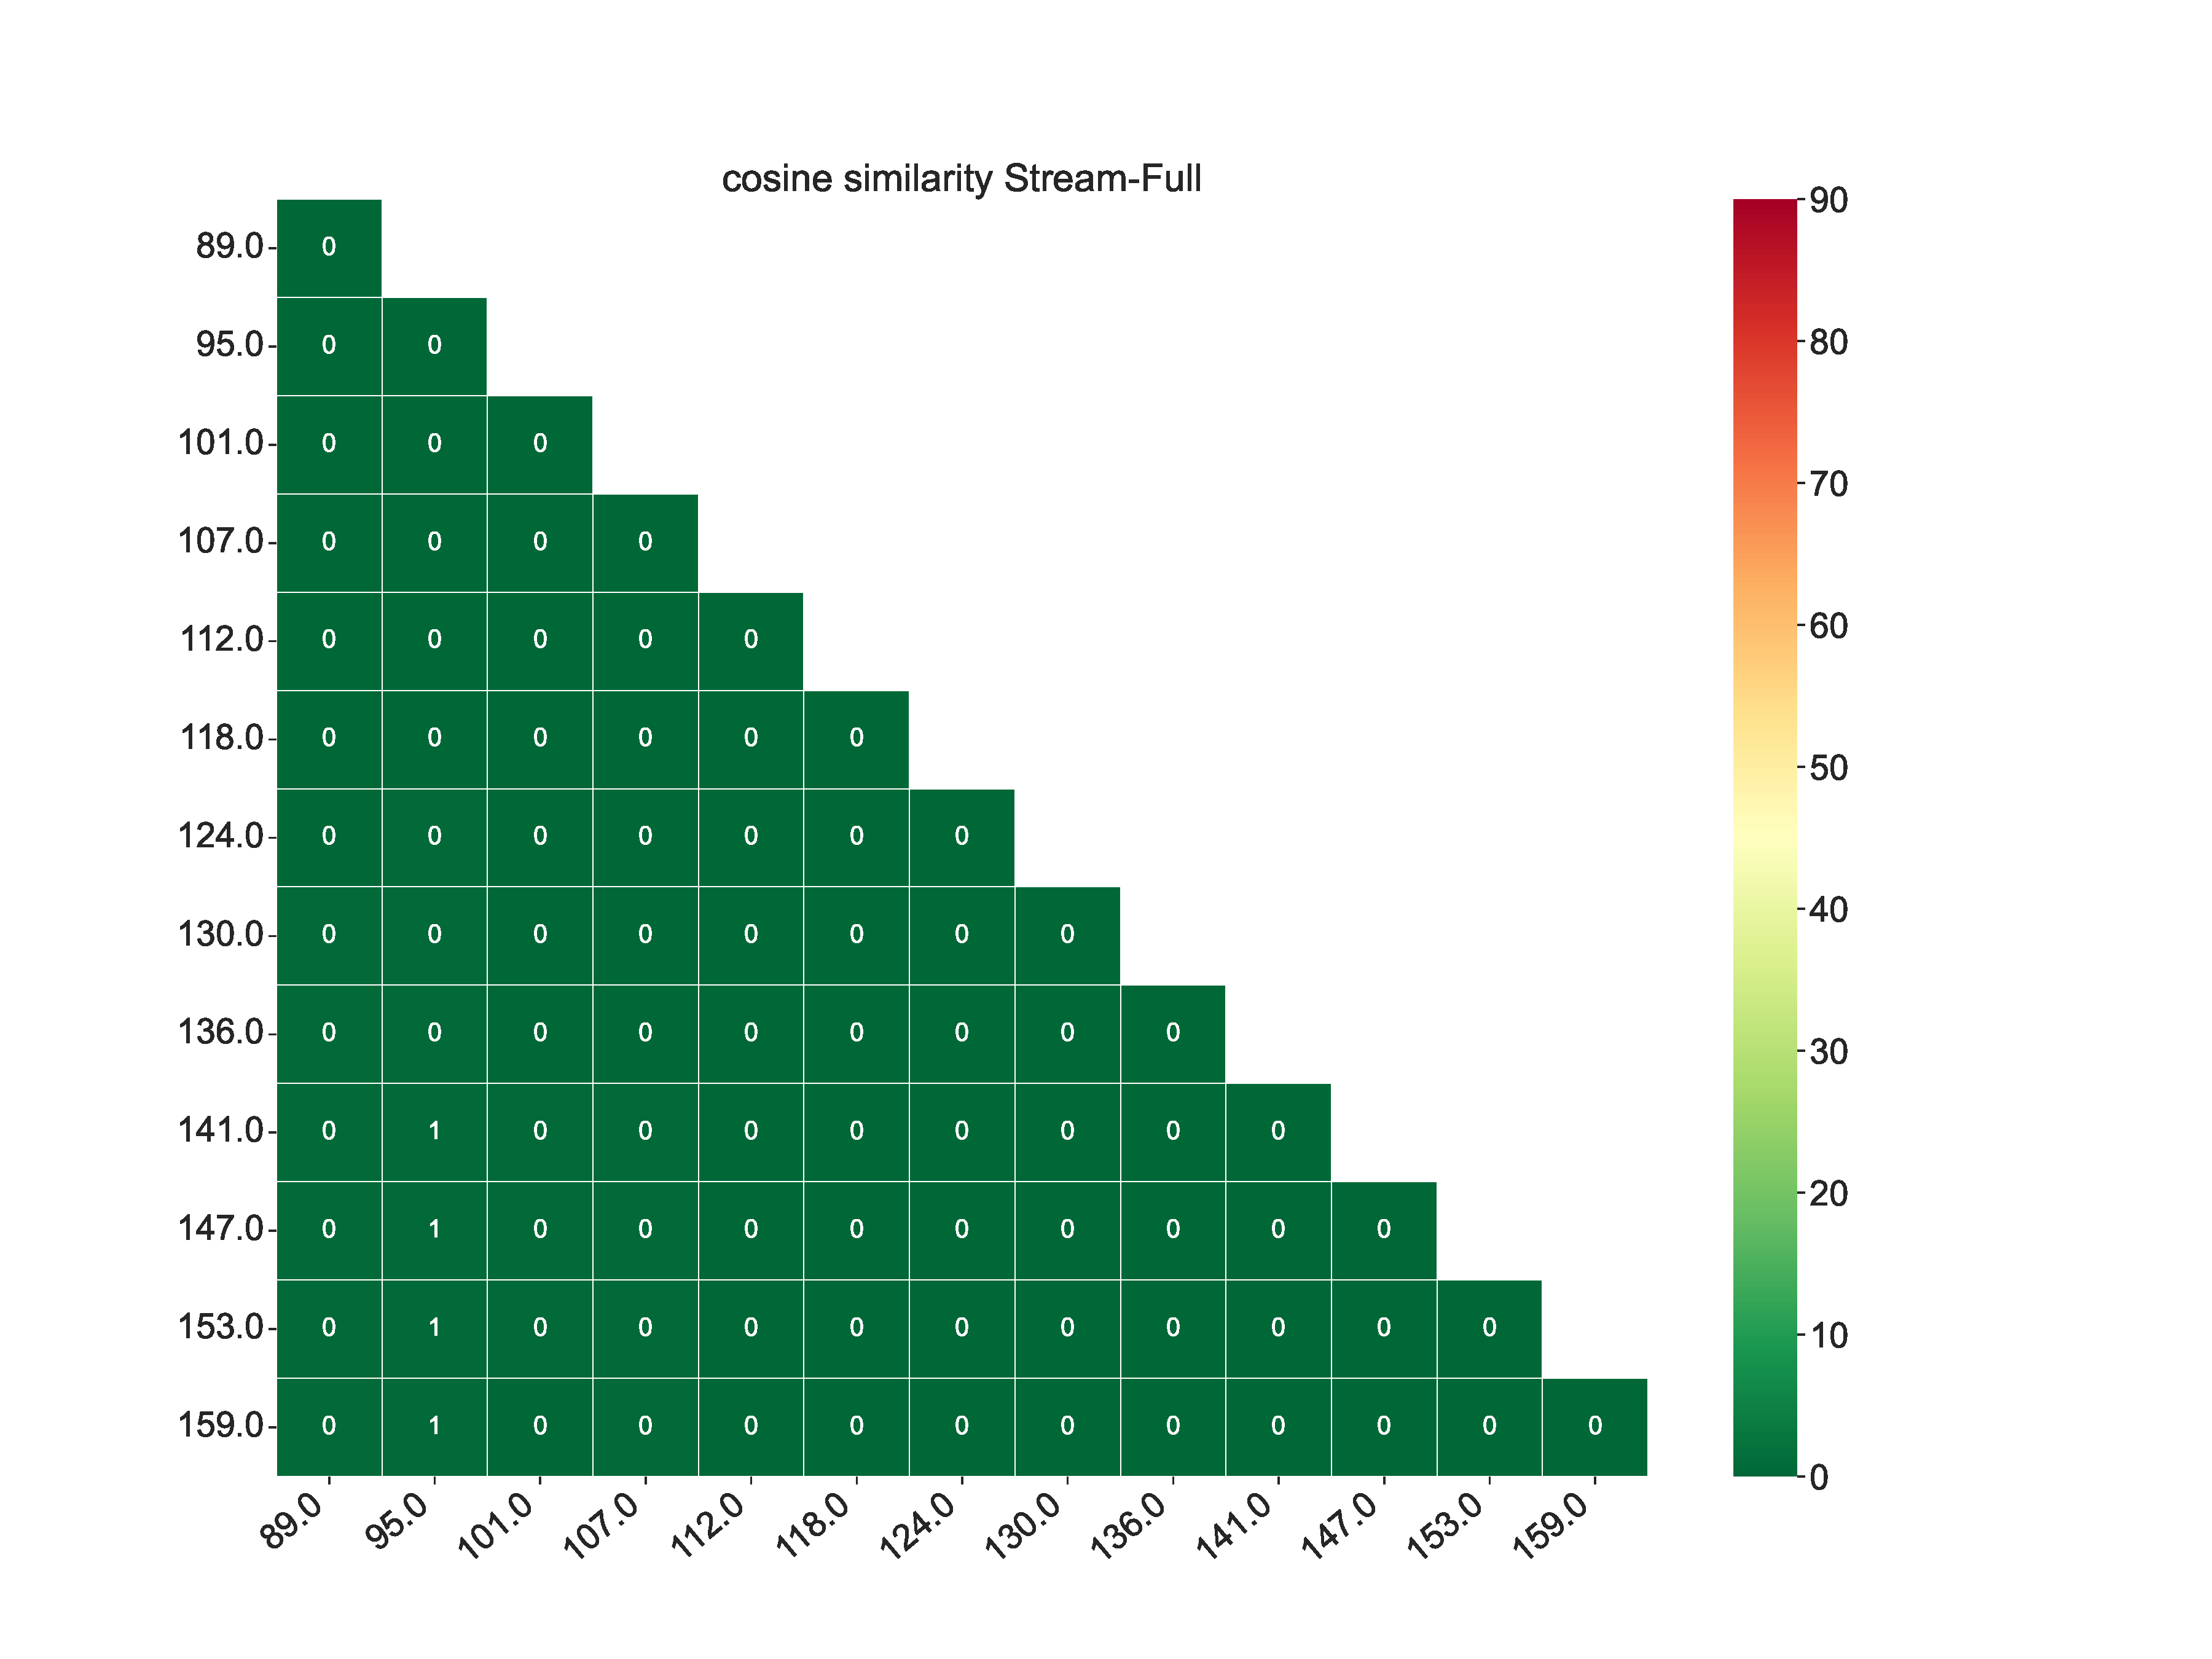
\includegraphics[width=\linewidth]{Figure/similarity_checks/cosine_similarity_Stream-Full.pdf}
        \caption{Cosine similarity of Stream-Full across all 13 power cap levels
                 (89\,W to 159\,W). The near-zero angles ($\leq 1^\circ$) across
                 all PCAP pairs confirm that the application's behavioral
                 fingerprint is invariant to power capping, supporting the use of
                 any power cap level for training without distributional shift.}
        \label{fig:calder_ones_stream_full_a}
    \end{subfigure}
    \hfill
    \begin{subfigure}[t]{0.48\linewidth}
        \centering
        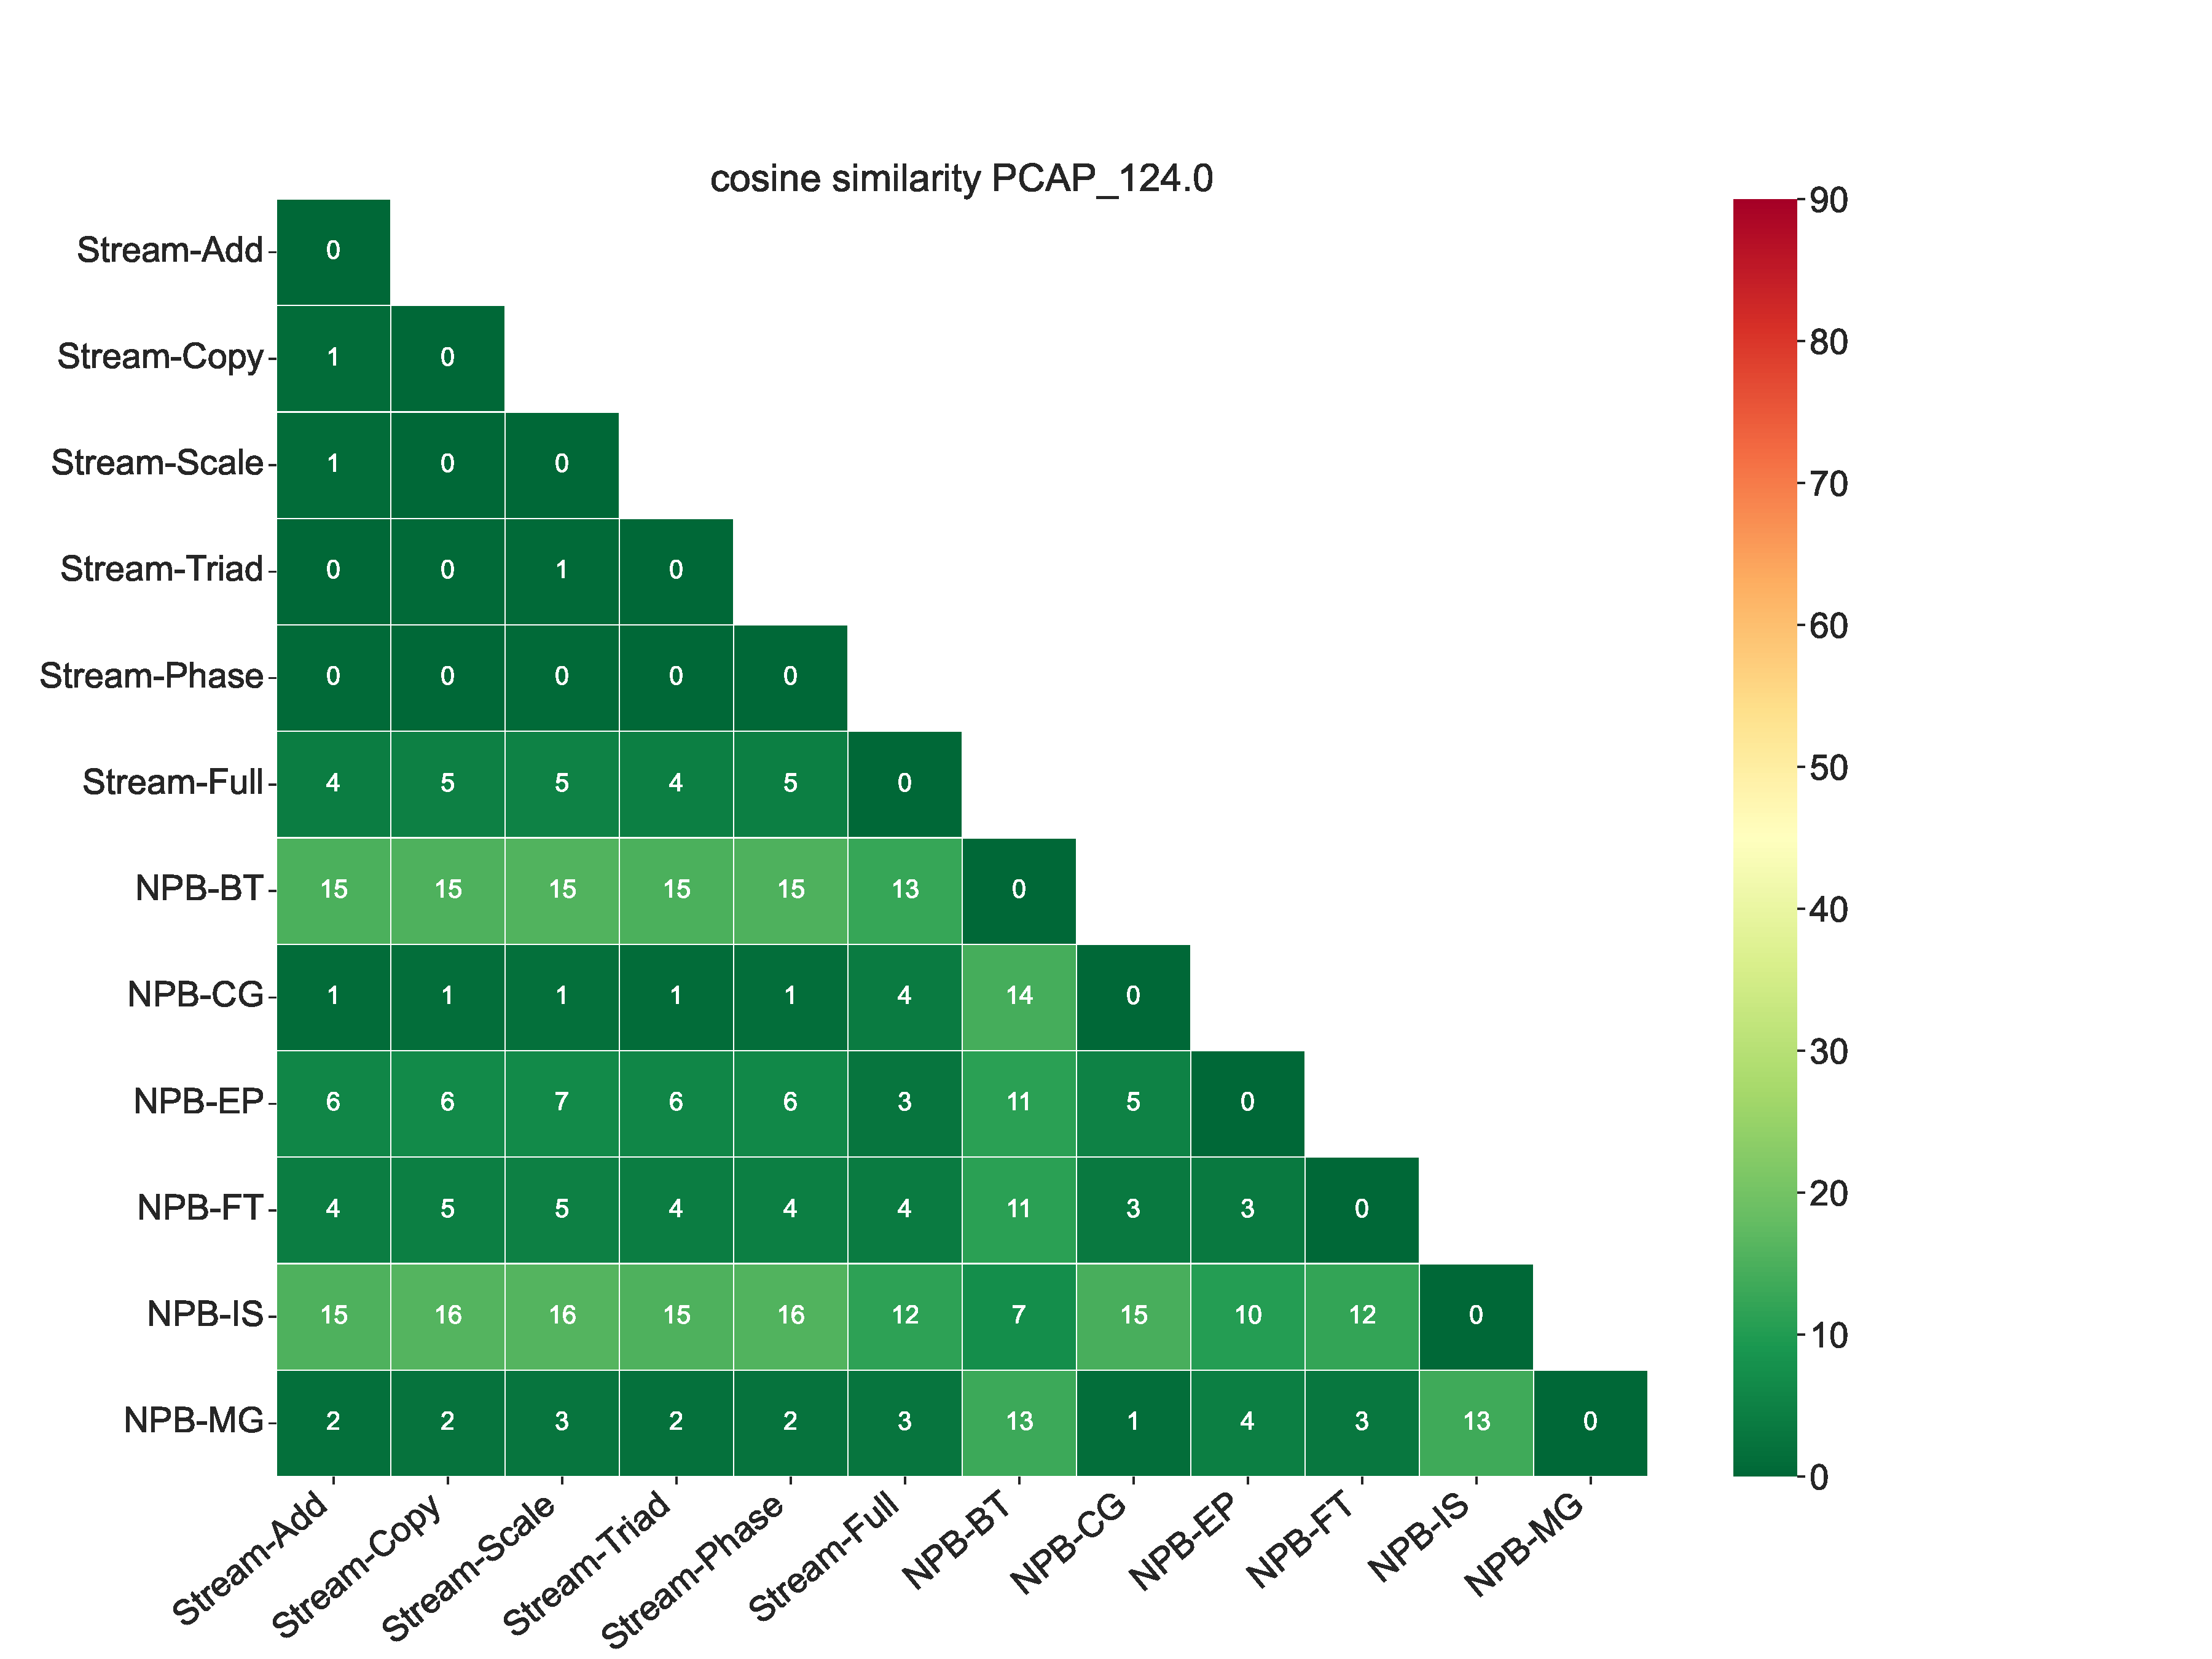
\includegraphics[width=\linewidth]{Figure/similarity_checks/cosine_similarity_PCAP_124.0.pdf}
        \caption{Cosine similarity between applications at a fixed power cap of
                 124\,W. Stream variants (Add, Copy, Scale, Triad) form a tight
                 cluster ($0$--$1^\circ$), while NPB-BT and NPB-IS are the most
                 behaviorally distinct ($13$--$16^\circ$), motivating their use
                 as out-of-distribution test workloads.}
        \label{fig:calder_ones_stream_full_b}
    \end{subfigure}

    \vspace{0.5em}

    \begin{subfigure}[t]{0.48\linewidth}
        \centering
        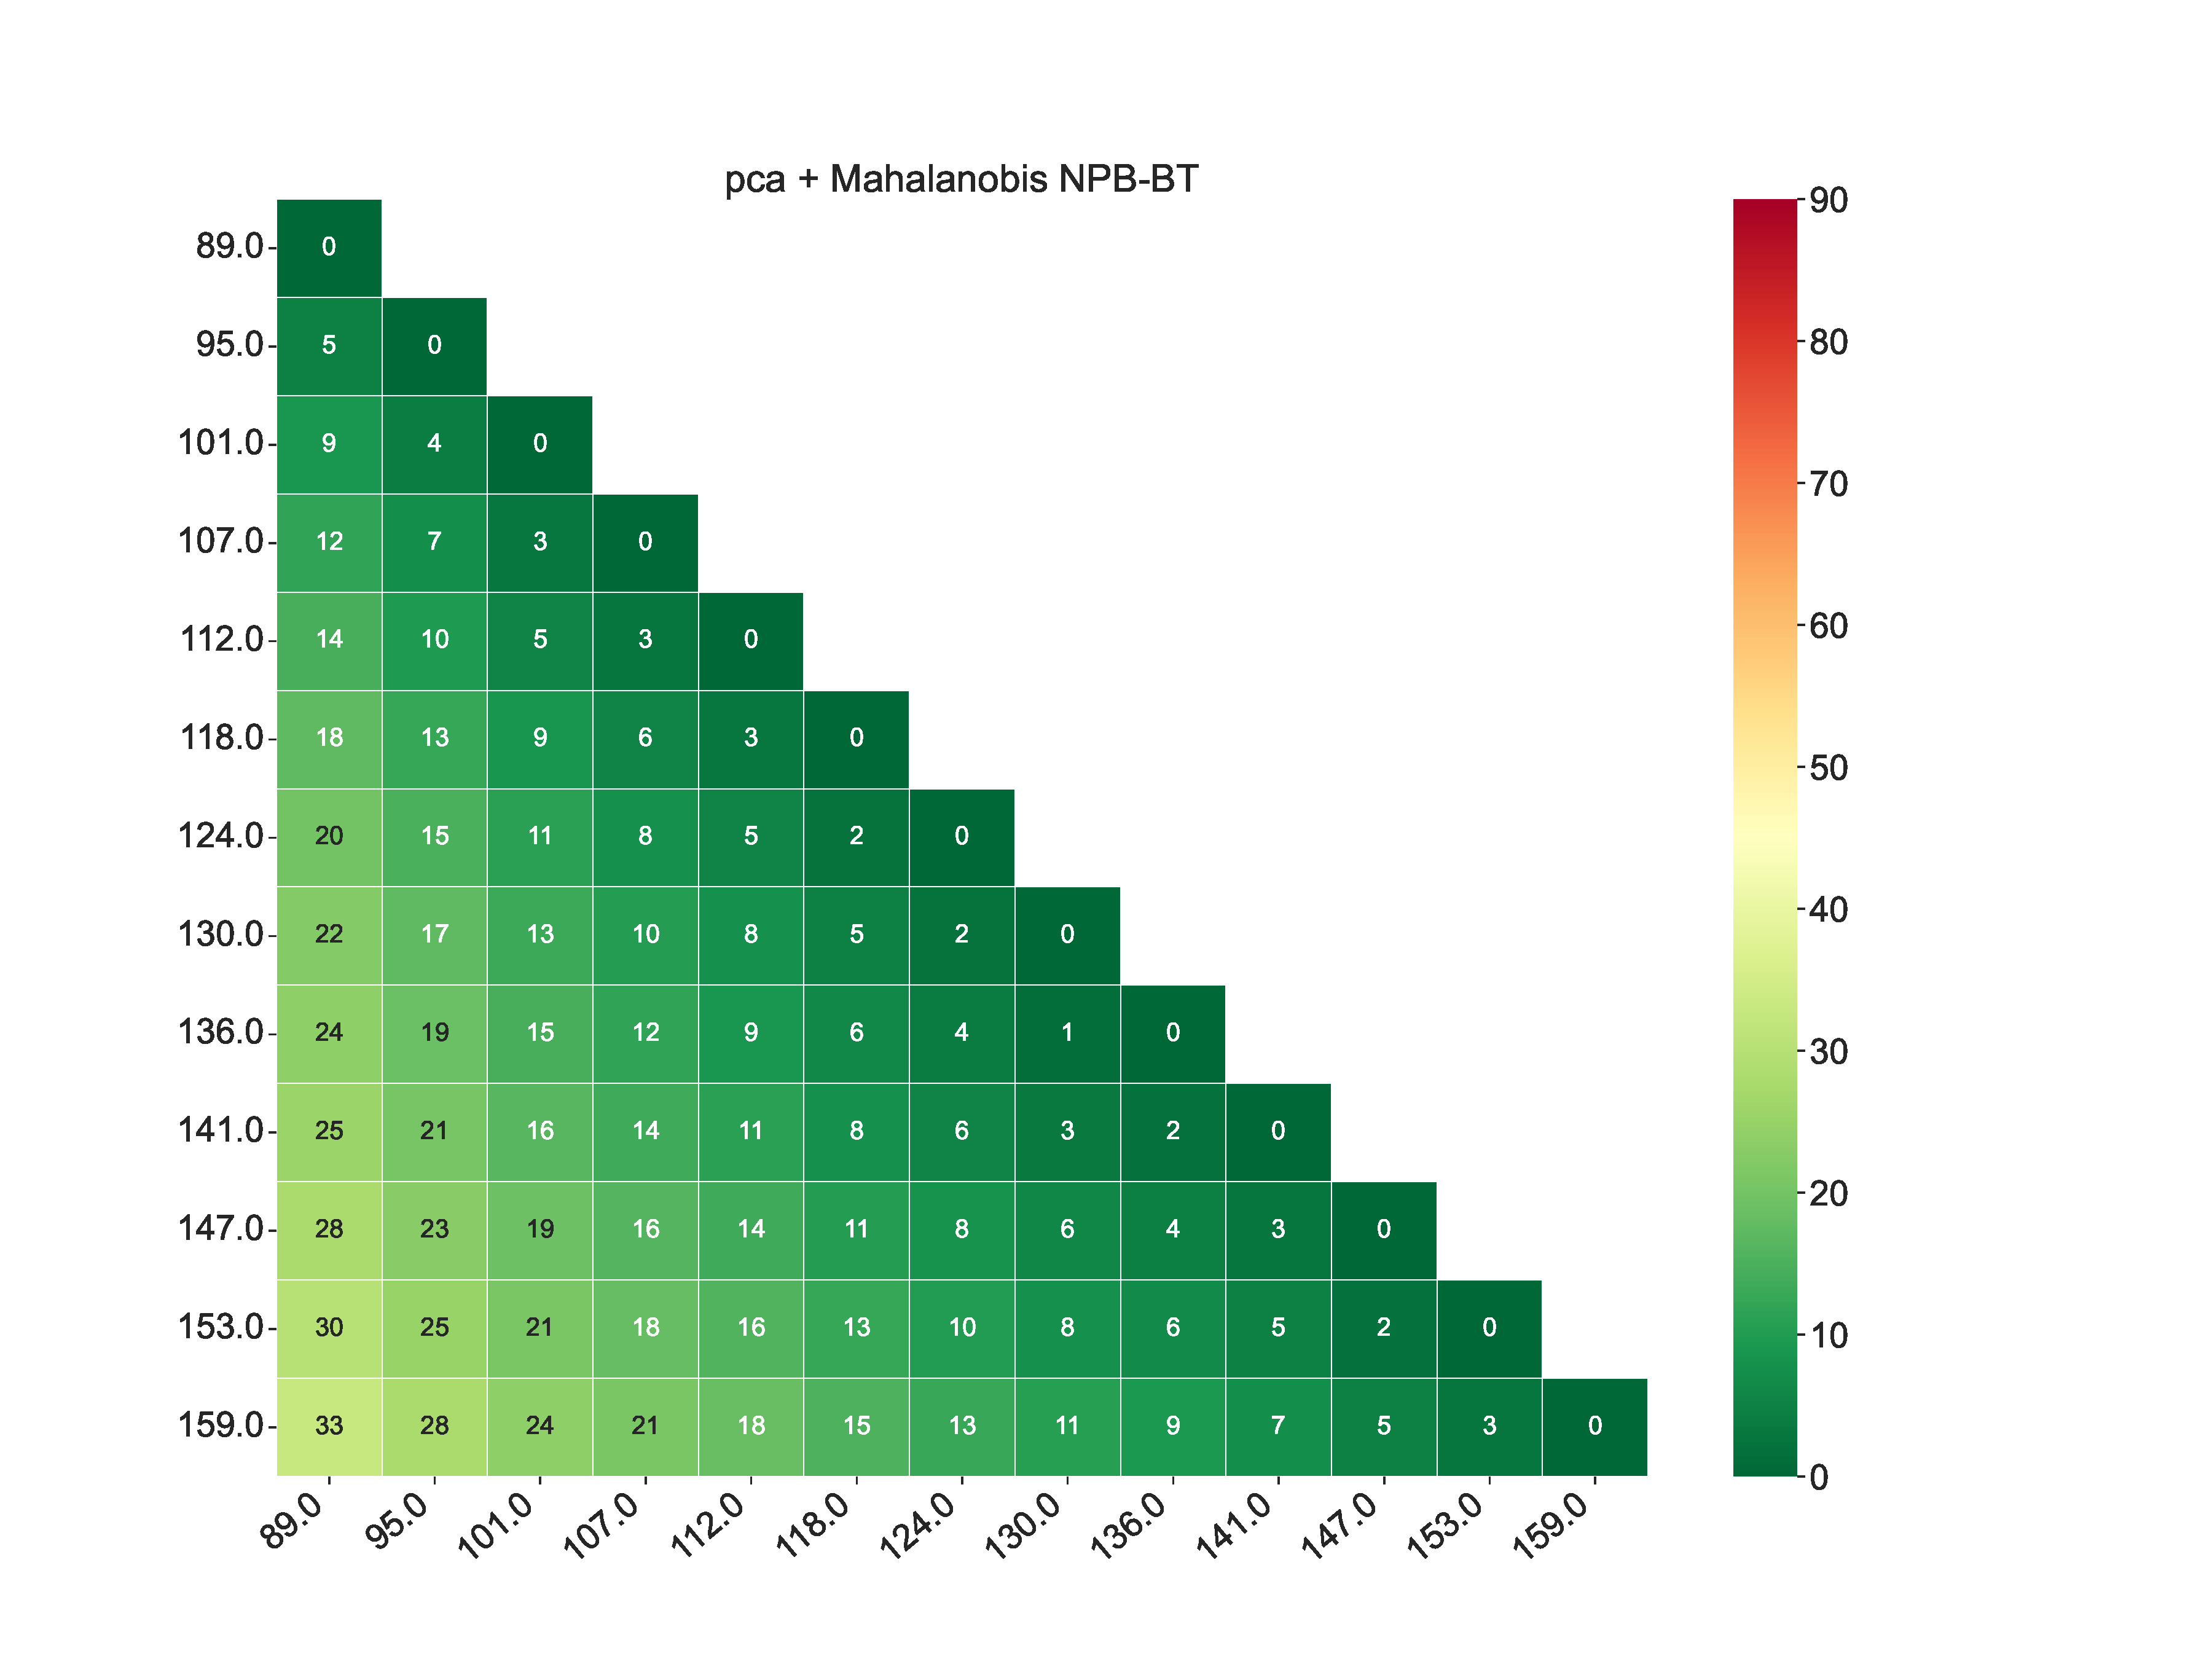
\includegraphics[width=\linewidth]{Figure/similarity_checks/pca_Mahalanobis_NPB-BT.pdf}
        \caption{PCA-reduced Mahalanobis distance between power cap conditions for
                 NPB-BT. The smooth monotonic increase (maximum distance of~33
                 between 89\,W and 159\,W) confirms that power capping
                 continuously shifts application throughput, justifying PCAP as a
                 continuous control dimension.}
        \label{fig:calder_pcap_bt}
    \end{subfigure}
    \hfill
    \begin{subfigure}[t]{0.48\linewidth}
        \centering
        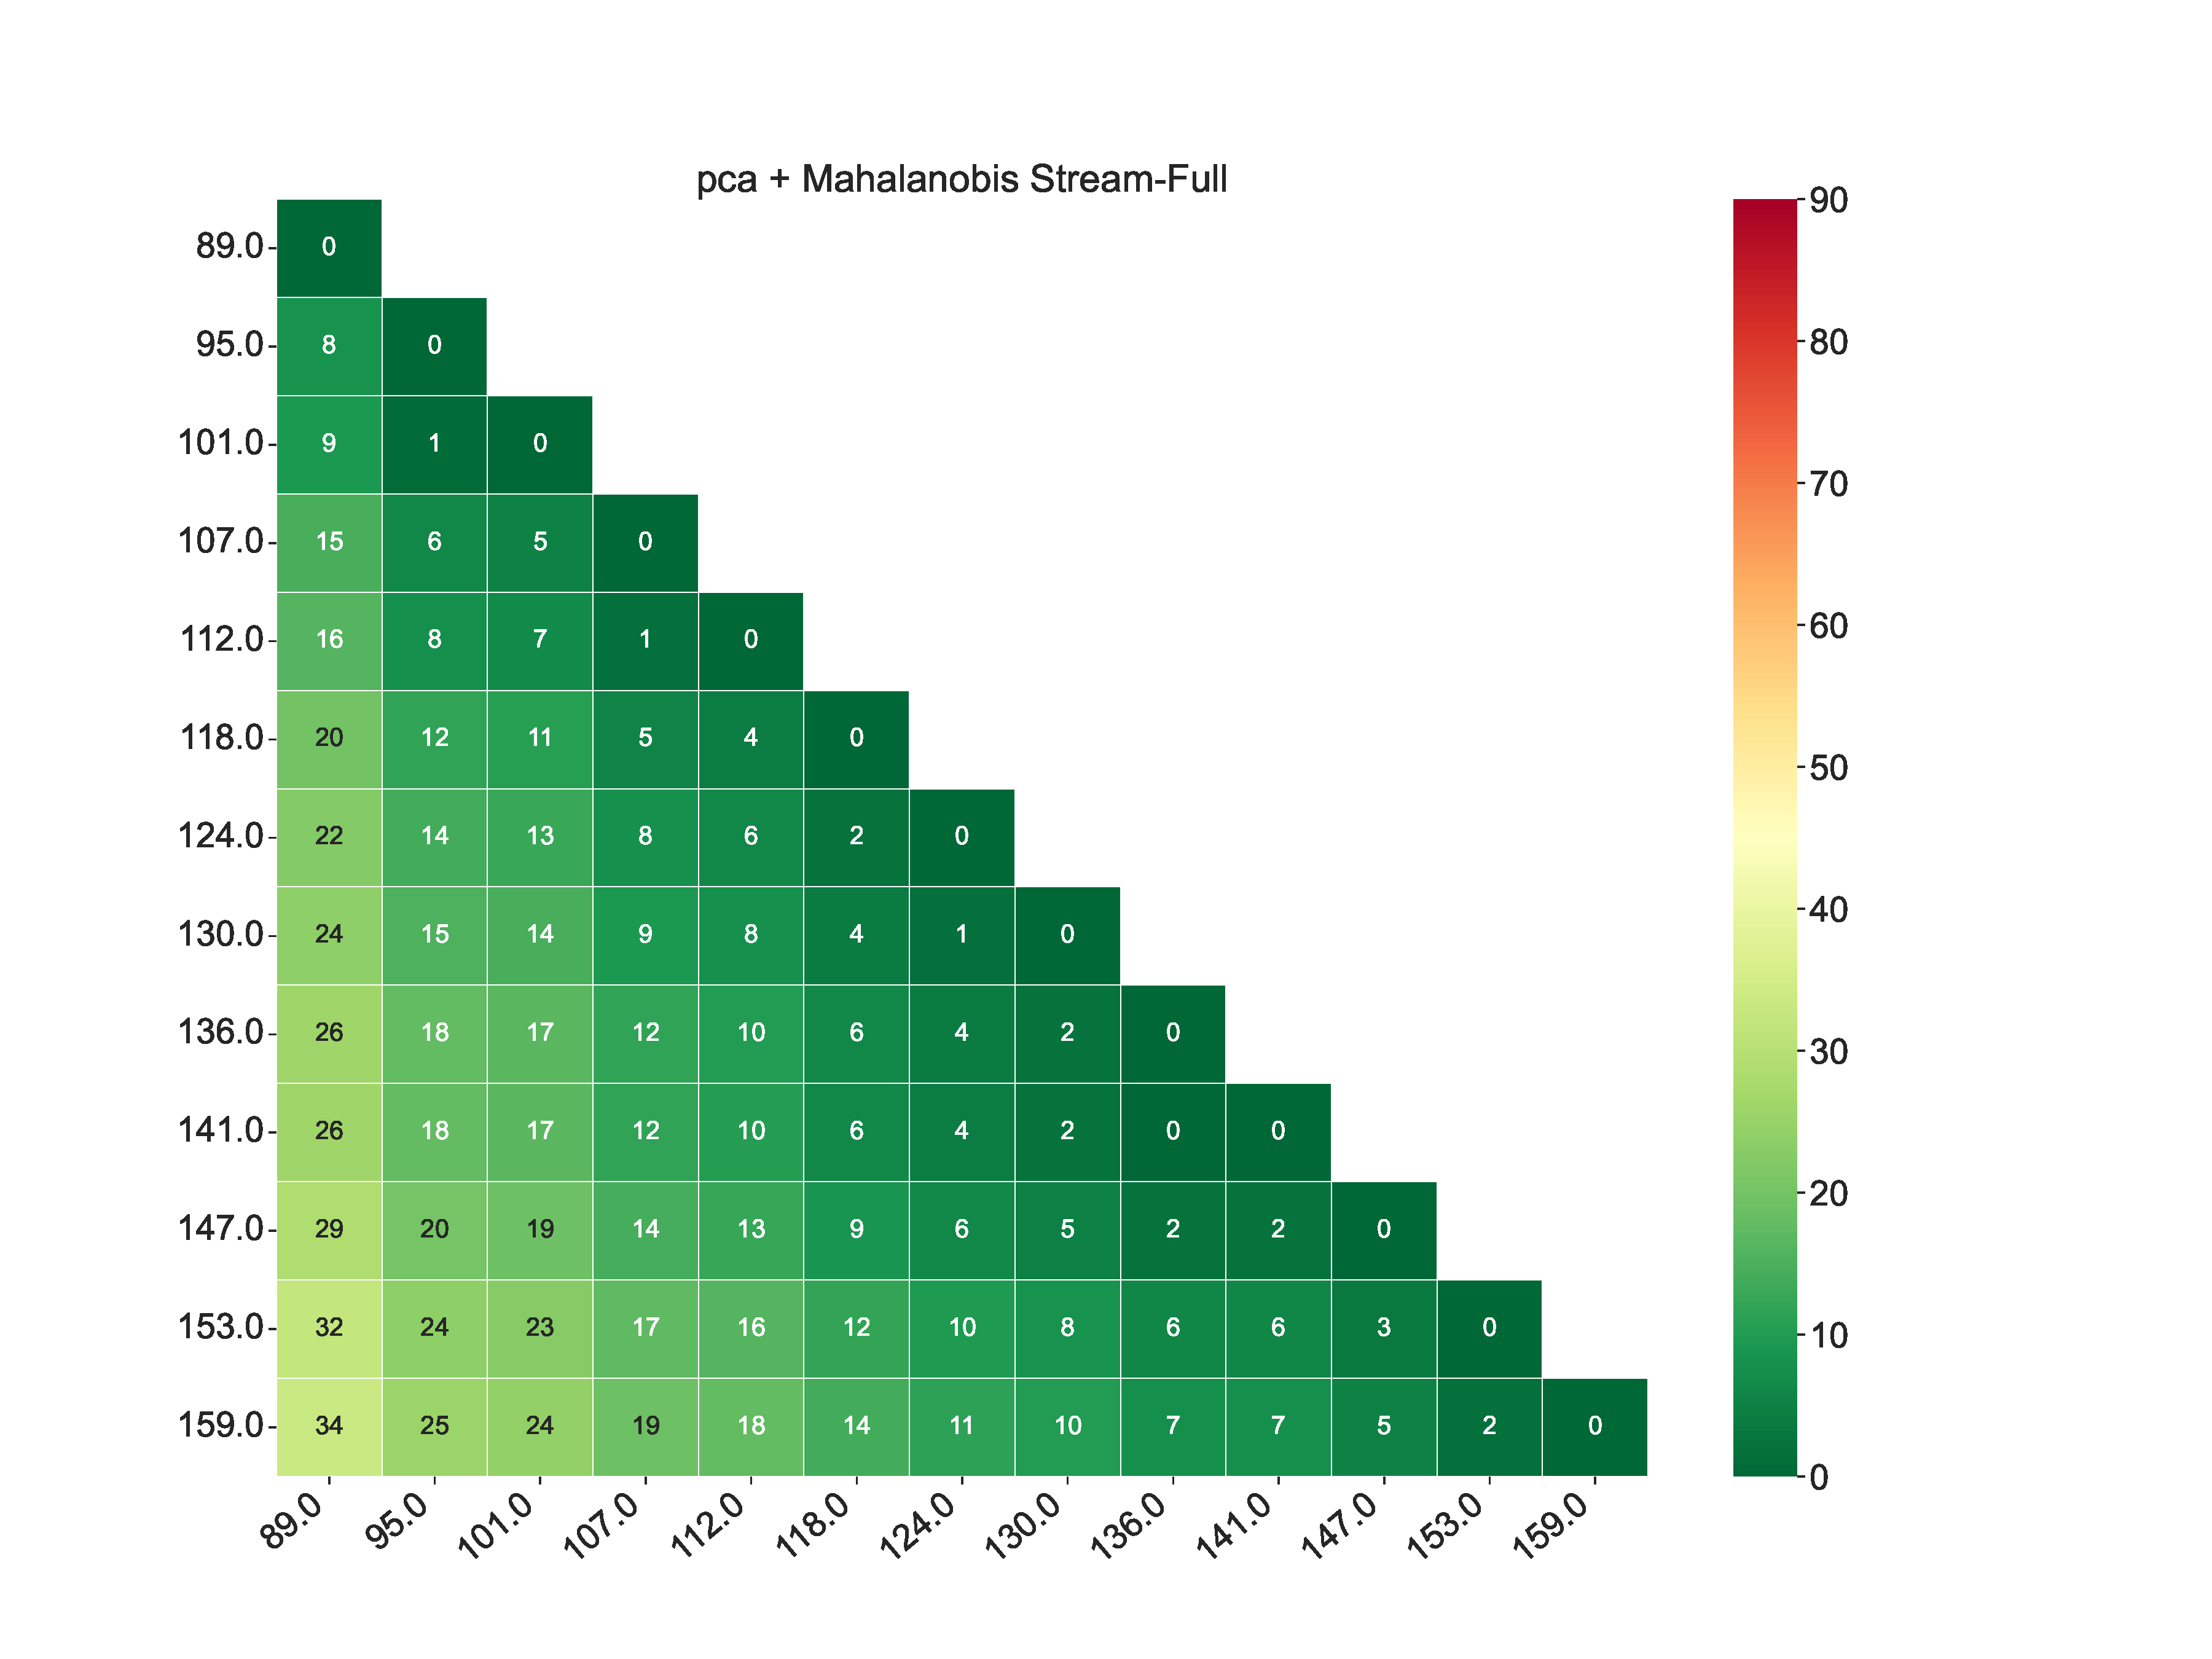
\includegraphics[width=\linewidth]{Figure/similarity_checks/pca_Mahalanobis_Stream-Full.pdf}
        \caption{PCA-reduced Mahalanobis distance between power cap levels for
                 Stream-Full. Behavior is nearly invariant across mid-to-high
                 caps (107\,W--159\,W, distance $\leq 10$) but diverges sharply
                 at the lowest cap (89\,W vs.\ 159\,W, distance~34), indicating
                 a saturation region at higher power budgets.}
        \label{fig:calder_pcap_stream_full}
    \end{subfigure}

    \caption{Application diversity and power-cap sensitivity across HPC workloads.
             Cosine similarity (top row) reveals that a single application's
             behavioral fingerprint is invariant to power capping but that
             different applications occupy distinct regions of feature space.
             PCA-based Mahalanobis distance (bottom row) captures the magnitude
             shifts in throughput induced by power capping, confirming a smooth
             and continuous response to PCAP adjustments.}
    \label{fig:combined_similarity}
\end{figure*}

Figure~\ref{fig:combined_similarity} summarises the four key observations.
Figure~\ref{fig:calder_ones_stream_full_a} shows that cosine similarity across all
13 power cap levels for Stream-Full remains below $1^\circ$, confirming that the
hardware behavioral fingerprint of a single application is invariant to power
capping.
This means data collected at any power cap level for a given application can be
included in the training set without introducing distributional shift; the policy
sees a consistent feature representation regardless of which PCAP levels were
sampled during data collection.

Figure~\ref{fig:calder_ones_stream_full_b} reveals the opposite picture across
applications: at a fixed power cap, Stream variants cluster tightly together
($0$--$1^\circ$), while NPB-BT and NPB-IS are substantially more distinct
($13$--$16^\circ$).
This cross-application diversity is the key criterion used to partition the
dataset: the five STREAM benchmarks, being behaviorally similar, are assigned
to the training split, while the four NPB benchmarks, being behaviorally
distinct from the training distribution, are reserved for out-of-distribution
testing to evaluate the generalization capability of the learned policy.

Figures~\ref{fig:calder_pcap_bt} and~\ref{fig:calder_pcap_stream_full} further
justify treating PCAP as a continuous control variable.
The Mahalanobis distance for NPB-BT increases monotonically with the separation
between power cap levels, reaching a maximum of~33 between the lowest (89\,W)
and highest (159\,W) caps.
Stream-Full shows a similar trend but with a saturation plateau at mid-to-high
caps, indicating that the policy does not need to distinguish finely between
power levels above approximately 107\,W.
Together, these results confirm that the training dataset can be constructed from
STREAM traces collected across the full PCAP range, and that the learned policy
is expected to encounter meaningfully different behavior when evaluated on NPB
workloads, providing a rigorous test of application-agnostic generalization.